\documentclass[../Main/main.tex]{subfiles}

\begin{document}
	\graphicspath{{../Time dependent equations/figs/}}
	\chapter{Richards' 2}
	In this chapter we discuss numerical solving algorithms for parabolic equations with non-linearities, such as Richards' equation \eqref{eq:richards}. 
	\section*{Time discretization}
	We start by considering the most famous parabolic equation, namely the heat equation:
	
	\begin{equation}\label{eq:heat equation}
		\begin{aligned}[c]
			\partial_t u - \nabla \cdot \pmb{K} \nabla u &= F \\
			u &= 0 \\
			\pmb{K}\nabla u &= g_N\\
			u &= u_0
		\end{aligned}
		\ \ \
		\begin{aligned}[c]
			x &\in \Omega  \\
			x &\in \partial \Gamma_D \\
			x &\in \partial \Gamma_N \\
			x &\in \Omega  
		\end{aligned}
		\ \ \
		\begin{aligned}
			t&\in (0,T] \\
			t&\in (0,T] \\
			t&\in (0,T] \\
			t&=0
		\end{aligned}
	\end{equation}
	
	We expect low regularity in time, so there is not much gained by using a higher order discretization in time. The two choices we have left is the forward euler(explicit) and the backward euler(implicit). The obvious choice is backward euler, as it is stable for long timesteps. This can be understood intuitively by considering the parabolic nature of the equation, the signals spread trough the domain instantaneously. A careful analysis time discretization of parabolic equations is done in (\cite{Knabner}, chapter 7).  Here it is shown that explicit schemes only are stable for time-step proportional to the square of the space step, whereas fully implicit schemes are stable for all time-steps. \par  Let $\left \{ t_n \right \}_n$ be a sequence of $N+1$ evenly spaced numbers from $0$ to $T$ and let $\tau = \frac{T}{N}$ be the time-step Then we state the semi-discrete version of \eqref{eq:heat equation} by exchanging the time derivative by a difference quotient $(\partial_t u)^n = \frac{u^n-u^{n-1}}{\tau}$. Note that this difference quotient is implicit because $u^n$ is not explicitly given by terms of the previous time-step
	\begin{equation}\label{eq:semidiscrete heat}
		\begin{aligned}[c]
			u^n - \tau \nabla \cdot \pmb{K} \nabla u^n &= \tau F^n+u^{n-1}\\
			u^n &= 0 \\
			\pmb{K}\nabla u &= g_N\\
			u^0 &= u_0
		\end{aligned}
		\ \ \
		\begin{aligned}[c]
			x &\in \Omega  \\
			x &\in \partial \Gamma_D \\
			x &\in \partial \Gamma_N \\
			x &\in \Omega  
		\end{aligned}
	\end{equation}
	Now we have an elliptic problem \eqref{eq:semidiscrete heat} for each time-step. This has almost the same structure as the elliptic model problem \eqref{eq:poisson} we solved in the previous chapters, the difference being that we have a $u^n$ term.
	\subsection*{Finite element approach}
	We are now ready to fit this problem into our finite element framework from chapter 2.
	The variational formulation of \eqref{eq:semidiscrete heat} is achieved as before by multiplying by test functions in $H^1_0(\Omega)$:
	\begin{equation}
		\begin{aligned}
			\text{find }u^n&\in V \text{ such that }\\
			\left \langle  u^n, v\right \rangle_0 + \tau \left \langle  \pmb{K} \nabla u^n, \nabla v \right \rangle_0 &=\tau \left \langle F^n,v\right \rangle_0 + \left \langle u^{n-1},v \right \rangle_0\\
			\text{for all }v&\in V
		\end{aligned}
	\end{equation}
	If we swap $V$ with  a finite dimensional subspace $V_h$, and write $u_h^n = \sum_{i = 1}^d (u_i^*)^n \phi_i $, as in the Galerkin FEM section, we end up with the system.
	\begin{equation}\label{eq:heat fem disc}
		\begin{aligned}
			\text{find }(\pmb{u}^*)^n&\in \mathbb{R}^d \text{ such that }\\
			\pmb{B}(\pmb{u}^*)^n+\tau\pmb{A}(\pmb{u}^*)^n &=\tau \pmb{F}^n +  \pmb{B}(\pmb{u}^*)^{n-1}
		\end{aligned}
	\end{equation}
	Where the \emph{stiffness matrix}, $\pmb{A}$, is as before. The matrix $\pmb{B}$ is often called the \emph{mass matrix} and is defined as $\pmb{B}_{i,j} = \int_{\Omega} \phi_i \phi_jdx$.
	\subsection*{Finite volume approach}
	As before we divide our domain $\Omega$ into control volumes $\left \{ \Omega_i \right \}_i$. One could write the heat equation\eqref{eq:heat equation} in conservation form on each control volume
	\begin{equation}
		\partial_t\int_{\Omega_i}u \ dx -\int_{\partial \Omega_i} \pmb{K}\nabla u \cdot \hat{\pmb{n}}\ dx = \int_{\Omega_i} F \ dx
	\end{equation}
	And discretize the first term with backward Euler. Or one could make sure the semi-discrete heat equation \eqref{eq:heat equation} holds for each control volume and use the divergence theorem. Both ways, we end up with
	\begin{equation}
		\int_{\Omega_i} u^n \ dx - \int_{\partial \Omega_i} \pmb{K}\nabla u^n \cdot \hat{\pmb{n}}\ dx = \int_{\Omega_i} F^n \ dx + \int_{\Omega_i} u^{n-1} \ dx
	\end{equation}
	As in chapter 3 we end up with a system of equations, where superscript $V$ is just to distinct between FVM and FEM.
	\begin{equation}\label{eq:heat fvm disc}
		(\pmb{B}^V + \tau \pmb{A}^V)\pmb{u}^n = \tau\pmb{F}^n + \pmb{B}^V\pmb{u}^{n-1}
	\end{equation}
	The matrix $\pmb{A}^V$ is as in chapter 3 with $\pmb{A}^V_{i,j}= \tilde{f}_{i,j}$ is the flux between cell $i$ and $j$. The matrix $\pmb{B}^V$ is diagonal with the entry $i$ being the volumes of the volume of cell $i$.

	If $\pmb{A}= \pmb{A}^V$, ie. that the discretization of the constitutive law is the same for both finite volume and finite element method. We can modify  the mass matrix and the load vector of the finite element method so that they become equivalent. To achieve this we define an interpolation operator as in (Cao and Wolmuth \cite{https://doi.org/10.1002/fld.1926},2009):
	\begin{definition}[Piecewise global interpolator]
		Let $\hat{I}_h$ be an operator that maps from the test space to functions that are piecewise continuous on each control volume.
		\begin{equation*}
			\hat{I}_h:C(\Omega)\rightarrow \left \{ v_h \in L^2(\Omega):v_h|_{\Omega_i} = K \right \}
		\end{equation*}
		And
		\begin{equation*}
			\hat{I}_h v = \sum_{i\in \mathcal{N}}v(x_i)\hat{I}_h\phi_i(x)
		\end{equation*}
		Where
		\begin{equation}
			\hat{I}_h\phi_i(x)=\left\{\begin{matrix}
				1 & \text{if } x\in \Omega_i\\ 
				0 & \text{otherwise}
			\end{matrix}\right.
		\end{equation}
	\end{definition}
	\begin{lemma}
		Suppose the stiffness matrix $\pmb{A}$ arising from the finite element discretization \eqref{eq:heat fem disc} is equivalent to the corresponding matrix in the finite volume discretization \eqref{eq:heat fvm disc} for some finite volume method. Then the Galerkin discretization 
		\begin{equation}\label{eq:lemma mass}
			\begin{aligned}
			\text{find }u_h^n &\in V_h\\
			\left \langle \hat{I}_h u_h^n,\hat{I}_h v_h \right \rangle_0 +\tau \left \langle  \pmb{K} \nabla u^n_h, \nabla v_h \right \rangle_0 &= \tau \left \langle F^n,\hat{I}_h v_h \right \rangle_0 + \left \langle \hat{I}_h u_h^{n-1},\hat{I}_h v_h \right \rangle_0 \\
			\forall v_h &\in V_h \\ 
			\text{ where } V_h = &\left \{ u_h \in C(\overline{\Omega}) : u_{h|K} \in P_1(K) \ \forall K \in \tau_h, u|_{\partial \Omega} = 0  \right \}
			\end{aligned}
		\end{equation}
		Is equivalent to the finite volume method \eqref{eq:heat fvm disc}
	\end{lemma}
	\begin{remark}
		Note that the use of the $\hat{I}_h$ operator is the same as using the trapezoidal quadrature rule to compute the inner product $\left \langle \phi_i,\phi_j \right \rangle_0$ instead of evaluating it exactly.
		This procedure is known as \textbf{mass lumping} and is shown in detail in (Baranger \cite{baranger1996connection},1995).
	\end{remark}
	\begin{proof}
		Let $u_h = \sum_i u_i^* \phi_i$, and let the test functions in \eqref{eq:lemma mass} be the basis functions $\left \{ \phi_j \right \}_j$, then we have 
		\begin{equation}
		\sum_{i\in \mathcal{N}} (u^*)^n_i (\left \langle \hat{I}_h\phi_i,\hat{I}_h\phi_j\right \rangle_0 +\tau \left \langle  \pmb{K} \nabla \phi_i, \nabla \phi_j \right \rangle_0) = \tau \left \langle F^n,\hat{I}_h \phi_j \right \rangle_0 + \sum_{i\in \mathcal{N}} (u^*)^{n-1}_i \left \langle \hat{I}_h \phi_i,\hat{I}_h \phi_j \right \rangle_0
		\end{equation}
		Now we see by the definition of the piecewise interpolator that we get:
		\begin{equation}
			\left \langle \hat{I}_h\phi_i,\hat{I}_h\phi_j\right \rangle_0 = \int_{\text{supp}(\phi_i)\bigcap\text{supp}(\phi_j)} 1 \ dx = |\Omega_i|
		\end{equation}
		This means that the mass matrix is a diagonal matrix as in the finite volume method. Similarly we have 
		\begin{equation}
			\left \langle F^n,\hat{I}_h \phi_j \right \rangle_0 = \int_{\Omega_j}F^n \ dx
		\end{equation}
	\end{proof}
	\section*{Equivalence between modified FEM and modified MPFA-L}	
	In this section we introduce finite volume L-method and finite element method for the time discretized problem \eqref{eq:semidiscrete heat}. 
	We saw in the section about the MPFA-L method that the interaction regions(L-triangles) may form a triangulation of our domain.
	Modifications are made to both methods so that we can exploit this fact and obtain equivalence. This section is adapted from \todo[inline]{add citation}
	\subsection{Modified MPFA-L method}
	First of all we assume that we have a parallelogram grid.
	\begin{figure}[H]\label{fig:paralellogram mesh}
		\centering
		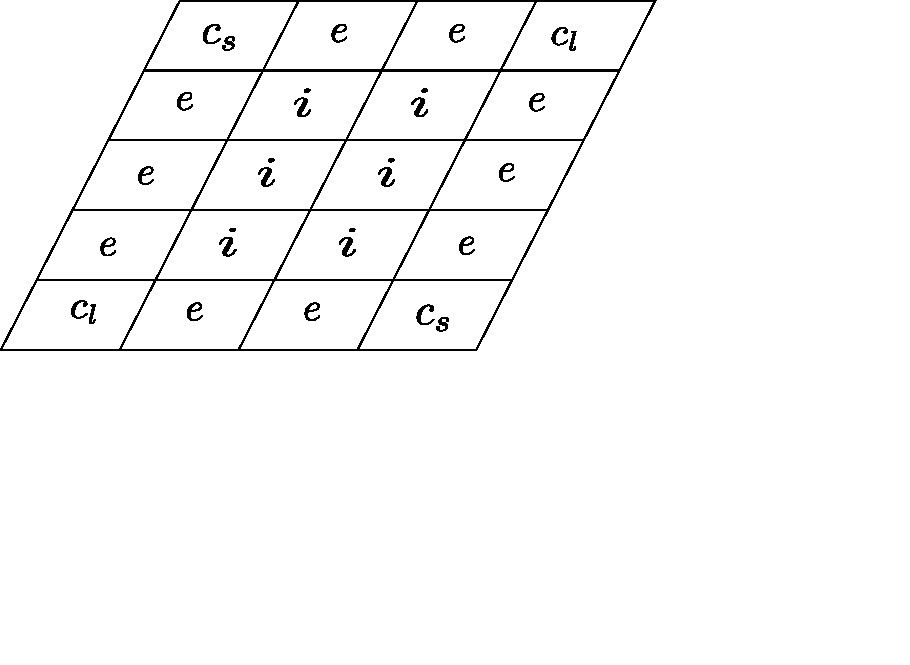
\includegraphics[width=1\textwidth]{paralellogram_mesh.pdf}
	\end{figure}

	To obtain a finite volume discretization one could write the heat equation\eqref{eq:heat equation} in conservation form on each control volume
	\begin{equation}
		\partial_t\int_{\Omega_i}u \ dx -\int_{\partial \Omega_i} \pmb{K}\nabla u \cdot \hat{\pmb{n}}\ dx = \int_{\Omega_i} F \ dx
	\end{equation}
	And discretize the first term with backward Euler. Or one could make sure the semi-discrete heat equation \eqref{eq:semidiscrete heat} holds for each control volume and use the divergence theorem. Both ways, we end up with
	\begin{equation}
		\int_{\Omega_i} u^n \ dx - \int_{\partial \Omega_i} \pmb{K}\nabla u^n \cdot \hat{\pmb{n}}\ dx = \int_{\Omega_i} F^n \ dx + \int_{\Omega_i} u^{n-1} \ dx
	\end{equation}
	The MPFA-L method deals with the second term, approximating the constitutive law. The other three terms are common to all control volume methods solving \eqref{eq:semidiscrete heat} and we will not make modifications or discuss them further.
	\par
	We will need to modify the Neumann boundaries, this is to be expected as finite element methods have degrees of freedom on the boundaries as opposed to finite volume methods. We will also see how we could enforce Dirichlet boundary conditions in a way that is equivalent to the finite element method. On the \textbf{interior} control volumes we use the original MPFA-L method already covered.
	\par
	Consider the control volume $y_1 y_6 y_4 y_3$. 
	\begin{figure}[H]
		\centering
		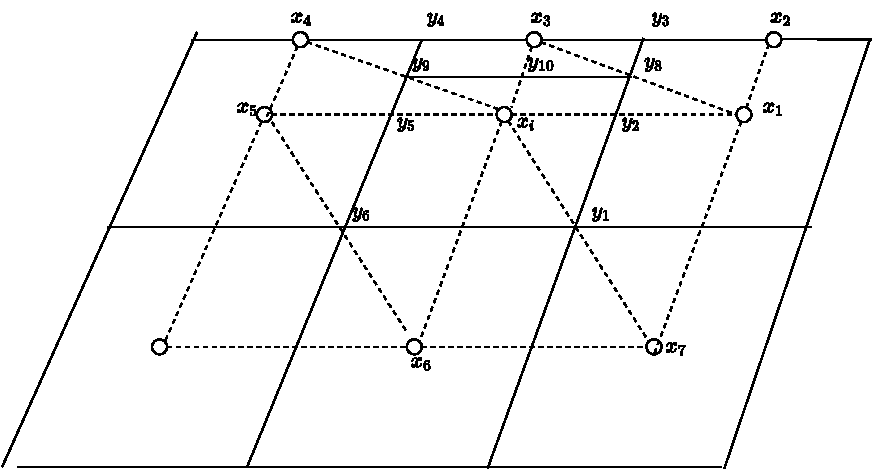
\includegraphics{modified_L_scheme.pdf}
		\caption{Control volumes in solid lines and interaction regions in dashed lines at the boundary.}
	\end{figure}
	\begin{figure}[H]\label{fig:volumepartition}
		\centering
		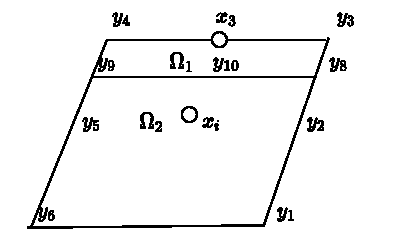
\includegraphics{volumepartition.pdf}
	\end{figure}
	For the \textbf{Neumann} boundary conditions, we split the cell into two, $y_1 y_6 y_9 y_8$ as $\Omega_2$ and $y_8 y_9 y_4 y_3$ as  $\Omega_1$. For the fluxes on $\Omega_2$ we have six interaction triangles and a normal seven point stencil. For the $\Omega_1$ we compute the flux trough $\overline{y_3 y_8}$ using $\triangle x_1 x_3 x_2$, the flux trough $\overline{y_8 y_{10}}$ using $\triangle x_1 x_i x_3$, for $\overline{y_{10}y_9}$ and $\overline{y_9 y_4}$ the L triangle  $\triangle x_i x_4 x_3$ is used. Finally the Neumann boundary condition is used at the the edge $\overline{y_4 x_3}$ and $\overline{x_3 y_3}$. We are not able to eliminate the unknown value at $x_3$ and it remains a degree of freedom, which makes sense if we want equivalence with finite element method.
	\par
	In the case of \textbf{Dirichlet} boundary conditions, we compute the fluxes into $y_1 y_6 y_4 y_3$ using seven L-triangles. The flux over the edge $\overline{y_3 y_1}$ are computed as the sum of the flux over $\overline{y_3 y_8}$, $\overline{y_8 y_2}$ and $\overline{y_2 y_1}$ using the L-triangles $\triangle x_1 x_3 x_2$, $\triangle x_1 x_i x_3$ and $\triangle x_1 x_7 x_i$ respectively. Similarly for the edge $\overline{y_6 y_4}$. For $\overline{y_1 y_6}$ we only use the two big L-triangles at the bottom. 
	\par 
	The flux over $\overline{y_4 y_3}$, at the boundary, we compute by balancing it by the other fluxes into the small control volume $\Omega_1$. Let $	f_{\overline{y_i y_j}}:= \int_{\overline{y_i y_j}}  \pmb{K}\nabla u \cdot \pmb{\hat{n}}\ dx $
	\begin{equation}\label{eq:K2}
		f_{\overline{y_4 y_3}} = f_{\overline{y_3 y_8}} + f_{\overline{y_8 y_{10}}}+f_{\overline{y_{10}y_9}}+f_{\overline{y_9 y_4}}
	\end{equation}
	The fluxes on the right hand side of \eqref{eq:K2} are computed as for the Neumann case.
	\subsection*{Modified finite element method}
	In this section we introduce a finite element method for solving \eqref{eq:semidiscrete heat}. We start by observing that by theorem \todo{add theorem in L-method chapter} the L-triangles form a triangulation. For the nodes of this triangulation $\tau_h$ we need some careful notation:
	\par 
	Let $\mathcal{N}_h^*$ be a set of indexes corresponding to all interior nodes of $\tau_h$, which are also the cell centers of the control volume mesh. This index set contains two disjoint sets $\mathcal{N}_h^* = \mathcal{N}_h^b \bigcup \mathcal{N}_h^i$, where superscript $i$ denotes the cell centers of the interior cells $i$ and $b$ the boundary cells $e$, see fig \ref{fig:paralellogram mesh}. the boundary cell center nodes are further diveded into three disjoint sets for edge cells, short corner cells and long corner cells: $\mathcal{N}^b_h = \mathcal{N}_h^e \bigcap \mathcal{N}_h^{c_l} \bigcap \mathcal{N}_h^{c_s}$. The Dirichlet and Neumann boundary nodes are denoted by $\mathcal{N}_h^D$ and $\mathcal{N}_h^N$ respectively. As with the cell-center index sets, the Neuman boundary index set is further divided into disjoint sets $\mathcal{N}_h^{N,e}\bigcap \mathcal{N}_h^{N,s}\bigcap\mathcal{N}_h^{N,l}\bigcap \mathcal{N}_h^{N,C_s}\bigcap\mathcal{N}_h^{N,C_l}$, where superscript $e$ denotes nodes at the middle of boundary cells, $s$ and $l$ denotes the nodes at the middle of the long and short corner cells and $C_s$ and $C_l$ denotes the node at the short and longer corner. Such that if we let $\mathcal{N}_h$ denote all the nodes of $\tau_h$ we get $\mathcal{N}_h = \mathcal{N}_h^*\bigcup \mathcal{N}_h^D \bigcup \mathcal{N}_h^N$.
	\par 
	As before one denotes by $V_h$ the linear ansatz space, see definition \ref{def:linear ansatz}. Similarly $\phi_i$ is the standard nodal basis function, where $i \in \mathcal{N}_h \setminus \mathcal{N}_h^D$.
	In addition to our global interpolation operator, definition \ref{def:global_interpolator}, we define:
	\begin{definition}[Piecewise global interpolator]
		Let $\hat{I}_h$ be an operator that maps from the test space to functions that are piecewise constant on each control volume.
		\begin{equation*}
			\hat{I}_h:C(\Omega)\rightarrow \left \{ v_h \in L^2(\Omega):v_h|_{\Omega_i} = K \right \}
		\end{equation*}
		And
		\begin{equation*}
			\hat{I}_h v = \sum_{i\in \mathcal{N}_h\setminus\mathcal{N}_h^d}v(x_i)\hat{I}_h\phi_i(x)
		\end{equation*}
		Where
		\begin{equation}
			\hat{I}_h\phi_i(x)=\left\{\begin{matrix}
				1 & \text{if } x\in D_i\\ 
				0 & \text{otherwise}
			\end{matrix}\right.
		\end{equation}
	\end{definition}
	\section*{Linearization}
	Now we have seen that the heat equation leads to a sequence of linear systems. In the same way, we expect that our non-linear Richards' equation \eqref{eq:richards} leads to a system of non-linear equations. We start by discussing this in a general setting
	\begin{equation}\label{eq:non-linear-problem}
		\text{find }x\in U \text{ such that }\pmb{f}(\pmb{x})=\pmb{0} \\ \text{ where } f:U\subset\mathbb{R}^n\rightarrow\mathbb{R}^n
	\end{equation}
	The solution in \eqref{eq:non-linear-problem} is called a \emph{root}, it is almost always found using an iterative method.\par 
	A common iterative scheme to solve \eqref{eq:non-linear-problem} is the \emph{Newton method}, let $D\pmb{f}(\pmb{x}_{j-1})^{-1}:\mathbb{R}^n\rightarrow\mathbb{R}^n$ be the Jacobian of $\pmb{f}(\pmb{x}_{j-1})$.
	\begin{equation}
		\pmb{x}_j = \pmb{x}_{j-1} -D\pmb{f}(\pmb{x}_{j-1})^{-1}\pmb{f}(\pmb{x}_{j-1})
	\end{equation}
	In one dimension a convergence proof i easily obtained by techniques from calculus, the following theorem is found in  slightly more detail in (Cheney\cite{Cheney}, chapter 3):
	\begin{theorem}
		Let $f''<2$ with $f(\overline{x})=0$ and $f'(x)> \delta \ \forall x \in B_{\epsilon}(\overline{x})$, then the Newton method is locally quadratic convergent:  For $x_0\in B_{\epsilon}(\overline{x})$ we have
		\begin{equation}
			| x_{j+1}-\overline{x}| \leq \frac{1}{\delta}|x_j - \overline{x}|^2< |x_j-\overline{x}|
		\end{equation}
	\end{theorem}
	\begin{proof}
		Define $e_n=x_n-\overline{x}$. Then we have by Taylor expansion
		\begin{equation}\label{eq:newton_taylor}
			0 = f(\overline{x})=f(x_j-e_j) = f(x_j)-f'(x_j)e_j + \frac{f''(\psi)e_j^2}{2}
		\end{equation}
		For some $\psi$ between $x_j$ and $\overline{x}$. Further we get by definition of the newton method
		\begin{equation}
			\begin{aligned}
				e_{j+1} = x_{j+1}-\overline{x} &= x_n-\frac{f(x_j)}{f'(x_j)}-\overline{x}\\
				&=e_j - \frac{f(x_j)}{f'(x_j)}\\ &= \frac{e_j f'(x_j)-f(x_j)}{f'(x_j)}
			\end{aligned}
		\end{equation}
		By the Taylor expansion around $x_j$, \eqref{eq:newton_taylor}, we get
		\begin{equation}
			e_{j+1} = \frac{e_j^2f''(\psi)}{2f'(x_j)}
		\end{equation}
	The assumptions on $f'$ and  $f''$ combined with $|e_0|<\delta$ give us the estimate
		\begin{equation}
			| e_{1} | \leq \frac{2}{2\delta}|e_0|^2<|e_0|
		\end{equation}
	By the same reasoning we get convergence
	\begin{equation}
		|e_{j+1}|<|e_j|
	\end{equation}
	And the quadratic convergence
	\begin{equation}
		| e_{j+1} | \leq \frac{1}{\delta}|e_j|^2
	\end{equation}
	\end{proof}
	For a similar result in more dimensions see (Knabner \cite{Knabner}, chapter 8). One apparent drawback of this method is that it's only locally convergent, ie. one needs to start the iteration in a neighbourhood of the root where the Jacobian is well defined. In practice one often solves the system
	\begin{equation}
		D\pmb{f}(\pmb{x}_{j-1})\pmb{\delta}_{j} = -\pmb{f}(\pmb{x}_{j-1})
	\end{equation}
	And then update the current iterate with $\pmb{x}_j = \pmb{x}_{j-1} + \pmb{\delta}_{j}$. One often end end up with a situation where the matrix $D\pmb{f}(\pmb{x}_{j-1})$ needs to be computed and assembled for every iteration. This may be computationally expensive. So Newtons method may be slow despite it's quadratic convergence, if it even converges.\par 
	A simpler approach is to swap the Jacobian with a diagonal matrix $L\pmb{I}$ such that 
	\begin{equation}
		L\pmb{\delta}_j = - \pmb{f}(\pmb{x}_{j-1})
	\end{equation}
	This is called the \emph{L-scheme}, and will be method we will use for linearization in this thesis. In one dimension it is easy to prove convergence:

	\begin{theorem}
		Let $f\in C(\mathbb{R})$ and $L>\sup_{x\in\mathbb{R}}f'(x)$, then the L-scheme converges linearly for all $x_0\in \mathbb{R}$.
	\end{theorem}
	\begin{proof}
		Define $e_j = e_j-\overline{x}$, then we get
		\begin{equation}
			e_{j+1} = x_j-\frac{f(x_j)}{L}-\overline{x}=e_j-\frac{f(x_j)}{L}
		\end{equation}
		We use the same trick as before with the Taylor expansion around the root.
		\begin{equation}
			0 = f(\overline{x}) = f(x_j-e_j) = f(e_j)-f'(\psi)e_j\Rightarrow e_j = \frac{f(x_j)}{f'(\psi)}
		\end{equation}
		Using this and the assumption on $L$ we get the estimate
		\begin{equation}
			|e_{j+1}|=|e_j(1-\frac{f'(\psi)f(x_j)}{f(x_j)L})|\leq|e_j||1-\frac{f'(\psi)}{L}|<|e_j|
		\end{equation}
	\end{proof}
	To see how this could be applied to parabolic PDE's we consider the equation:
	
	
	
	
	We will first consider the equation
	\begin{equation}\label{eq:richards simple}
		\begin{aligned}[c]
			\partial_t \theta(u) - \nabla \cdot \kappa (u) \nabla u &= F \\
			u &= g \\
			u &= u_0
		\end{aligned}
		\ \ \
		\begin{aligned}[c]
			x &\in \Omega  \\
			x &\in \partial \Omega \\
			x &\in \Omega  
		\end{aligned}
		\ \ \
		\begin{aligned}
			t&\in (0,T] \\
			t&\in (0,T] \\
			t&=0
		\end{aligned}
	\end{equation}
	Which is similar to Richards' equation \eqref{eq:richards}, only without the gravity. We proceed as before by backward euler in time and we then discretize the elliptic PDE with the Galerkin discretization with mass lumping \eqref{eq:lemma mass}. We then get:
	\begin{equation}
		\begin{aligned}
			\text{find }u_h^n&\in V_h\\
			\left \langle \hat{I}_h \theta(u_h^n),\hat{I}_h v_h \right \rangle_0 +\tau \left \langle \kappa(u_h^n) \nabla u^n_h, \nabla v_h \right \rangle_0 &= \tau \left \langle F^n,\hat{I}_h v_h \right \rangle_0 + \left \langle \hat{I}_h u_h^{n-1},\hat{I}_h v_h \right \rangle_0 \\
			\text{for all }v_h &\in V_h
		\end{aligned}
	\end{equation}
	We can then linearize $\theta(u^n_h)$ with the L-method, such that we en up with: Given $u^{n-1}_h$ and $u^{j-1,n}_h$ find $u^{j,n}_h$ such that:
	\begin{equation}
		\begin{aligned}
			\left \langle \hat{I}_h \theta(u^{n,j-1}_h),\hat{I}_h v_h \right \rangle_0 &+ L \left \langle \hat{I}_h u^{j,n}_h -  \hat{I}_h u^{j-1,n}_h,\hat{I}_h v_h \right \rangle_0 + \tau \left \langle \kappa(u_h^{j-1,n})\nabla u^{j,n}_h,\nabla v_h \right \rangle \\=\tau \left \langle F^n,\hat{I}_h v_h \right \rangle_0 &+ \left \langle \hat{I}_h u_h^{n-1},\hat{I}_h v_h \right \rangle_0 
		\end{aligned}
	\end{equation}
	\begin{theorem}
		Assume $\theta$ and $\kappa$ monotone ...
	\end{theorem}
	\section*{Equivalence between MPFA-L method and modified finite element method}
	In this section we prove the equivalence for the elliptic model problem \eqref{eq:elliptic model} on inhomogeneous media discretized by a parallelogram grid.
	\begin{equation}\label{eq:elliptic model}
		\begin{aligned}[c]
			- \nabla \cdot \pmb{K} \nabla u(x) &= F(x) \\
			u(x) &= 0 \\
			\pmb{K}\nabla u(x) &= g_N
		\end{aligned}
		\ \ \
		\begin{aligned}[c]
			x &\in \Omega  \\
			x &\in \Gamma_D \\
			x &\in \Gamma_N
		\end{aligned}
	\end{equation}	
	We 
	
\end{document}